This chapter continues looking at the case where the MDP models are
large state space. In the previous chapter we looked at
approximating the value function. In this chapter we will consider
learning directly a policy and optimizing it.

\AT{Move to later} The main advantages and disadvantages of policy optimization (rather
than value function approximation) are the following:
\begin{enumerate}
\item
Continuous action space. In such a case the policy optimization
method is the most natural and the one which is used in practice
(for applications such as robotics).
\item
Convergence: While the policy optimization would normally converge,
it will most likely converge to a local optimum.
\item
High dimensional spaces: It can be fairly effective in selecting the
actions (in contrast to learning accurate values).
\item
Evaluation time would typically be longer (compared to value
function approaches).
\item
Stochastic Policy: allows naturally to have a stochastic policy.
\end{enumerate}

\section{Problem Setting}

To describe the problem formally, we shall make an assumption about the policy structure and the optimization objective, as follows. 
% We will assume that each state $\state$ has an encoding
% $\phi(\state)\in \mathbb{R}^{d_1}$. 
The policy will have a
parametrization $\theta\in \mathbb{R}^{d}$, and we denote by 
$\policy(\action|\state,\theta)$ the probability of
selecting action $\action$ when observing state $\state$, and having a policy parametrization
$\theta$. 

For technical ease, we consider a stochastic shortest path objective:
\[\Value^\policy(\state) = \mathbb E^{\pi }\left[\left.\sum\limits_{\ttime = 0}^\termtime {{\reward_\ttime}} \right|\state_0 = \state\right],\]
where $\termtime$ is the termination time, which we will assume to bounded with probability one.
We are given a distribution over the initial state of the MDP, $\initdist(\state_0)$, and define $J(\theta) \triangleq \mathbb{E}\left[ \Value^\policy(\state_0)\right] = \initdist^\top \Value^\policy$ to be the expected value of the policy (where the expectation is with respect to $\initdist$).

The optimization problem we consider is:
\begin{equation}\label{eq:policy_opt}
\theta^* = \arg\max_\theta J(\theta).
\end{equation}

% where $J(\theta) \triangleq \Value^\policy(\state_0)$ is the
% expected return of the policy $\policy(\cdot|\cdot,\theta)$ from the
% initial state $\state_0$.
%
This maximization problem can be solved in multiple ways. We will
mainly explore gradient based methods.

In the setting that the MDP is not known, we shall assume that we are allowed to simulate `rollouts' from a given policy, $\state_0,\action_0,\reward_0,\dots,\state_\termtime, \action_\termtime, \reward_\termtime$, where $\state_0 \sim \initdist$, $\action_\ttime\sim \policy(\cdot|\state_\ttime,\theta)$, and $\state_{\ttime+1} \sim \transitionkernel (\cdot | \state_\ttime, \action_\ttime)$. We shall devise algorithms that use such rollouts to modify the policy parameters $\theta$ in a way that increases $J(\theta)$.

\section{Policy Representations}
We start by giving a few examples on how to parameterize the policy.
\paragraph{Log linear policy} We will assume a feature encoding
of the state and action pairs, i.e., $\phi(\state,\action)\in \mathbb{R}^{d}$. Given the parameter $\theta$, The linear part will compute $\mu(\state,\action)=\phi(\state,\action)^\top \theta$. Given the values of $\mu(\state,\action)$ for each $\action\in \Actions$, the policy selects action $\action$ with probability proportional to
$e^{\mu(\state,\action)}$. Namely,
\[
\policy(\action|\state,\theta)=
\frac{e^{\mu(\state,\action)}}{\sum_{b\in
\Actions}e^{\mu(\state,b)}}
\]
Note that this is essentially a soft-max selection over $\mu(\state,\action)$.

\paragraph{Gaussian linear policy} This policy representation applies when the action
space is a real number, i.e., $\Actions=\mathbb{R}$. The encoding is of states, i.e., $\phi(\state)\in \mathbb{R}^{d}$, and the actions are any real number. Given a state $\state$
we compute $\mu(\state)=\phi(\state)^\top\theta$. We select an
action $\action$ from the normal distribution with mean
$\mu(\state)$ and variance $\sigma^2$, i.e.,
$\mathcal{N}(\mu(\state),\sigma^2)$. (The Gaussian policy has an additional
parameter $\sigma$.)

\paragraph{Non-linear policy} Note that in both the log linear and Gaussian linear policies above, the dependence of $\mu$ on $\theta$ was linear. It is straightforward to extend these policies such that $\mu$ depends on $\theta$ in a more expressive and non-linear manner. A popular parametrization is a feed-forward neural network, also called a multi-layered perceptron (MLP). An MLP with $d$ inputs, 2 hidden layers of sizes $h_1$, $h_2$, and $k$ outputs has parameters $\theta_0 \in \mathbb{R}^{d \times h_1}$, $\theta_1 \in \mathbb{R}^{h_1 \times h_2}$, $\theta_2 \in \mathbb{R}^{h_2 \times k}$. The MLP computes $\mu\in \mathbb{R}^{k}$ as follows:
\begin{equation*}
    \mu(\state) = \theta_2^T f_{nl}\left(\theta_1^T\left( f_{nl}\left(\theta_0^T \phi\left(\state \right)\right)\right)\right) \in \mathbb{R}^{k},
\end{equation*}
where $f_{nl}$ is some non-linear function that is applied element-wise to each component of a vector, for example the Rectified Linear Unit (ReLU) defined as $\text{ReLU}(x) = \max(0, x)$. Once $\mu$ is computed, selecting an
action proceeds similarly as above, e.g., by sampling from the normal distribution with mean
$\mu(\state)$ and variance $\sigma^2$.

\paragraph{Simplex policy} This policy representation will be used mostly for pedagogical reasons, and can express any Markov stochastic policy. For a finite state and action space, let $\theta \in [0,1]^{\States \times \Actions}$, and denote $\theta_{\state,\action}$ the parameter corresponding to state $\state$ and action $\action$. We define $\policy(\action|\state,\theta) = \frac{\theta_{\state,\action}}{\sum_{\action'} \theta_{\state,\action'}}$. Clearly, any Markov policy $\tilde{\policy}$ can be represented by setting $\theta_{\state,\action} = \tilde{\policy}(\action|\state)$.

\subsection{Motivation for Stochastic Policies}
\AT{There's also an algorithmic motivation directly related to the policy gradient algorithms (exploration, and a well defined policy gradient) - do we want to discuss this?}
The policy examples above are stochastic. However, we have seen that the optimal policy in an MDP is deterministic, so
what benefit can be in considering a stochastic policy?

The main benefit is in situations where there is a
miss-specification of the model. The main issue is that the state
encoding might create a system which is not Markovian anymore, by
coalescing certain states which have identical encoding. We will
give two example of this phenomena.

\paragraph{Aliased Grid-world}\ \\
Consider the example in Figure~\ref{fig:L9-grid-world}. The green
state is the good goal and the red ones are the bad. The encoding of
each state is the location of the walls. In each state we need to
choose a direction. The problem is that we have two states which are
indistinguishable (marked by question mark).

It is not hard to see that any deterministic policy would fail from
some start state (either the left or the right one). Alternatively,
we can use a randomized policy in those states,with probability half
go right and probability half go left. For such a policy we have a
rather short time to reach the green goal state (and avoid the red
states).

The issue here was that two different states had the same encoding,
and thus violated the Markovian assumption. This can occur when we
encode the state with a small set of features, and some (hopefully,
similar) states coallesce to a single representation.

\begin{figure}
  % Requires \usepackage{graphicx}
  \begin{centering}
  \includegraphics[width=0.5\textwidth]{figures/L9-grid-world.png}\\
  \caption{Grid-world example }\label{fig:L9-grid-world}
  \end{centering}
\end{figure}

\paragraph{Zero-sum games}\ \\
The MDP model was not designed for interactive zero-sum games,
however, in many of the applications we saw, we train a policy to
play a board game (such as backgammon). Any board game is an
instance of a zero-sum game, since if one player wins the other
loses. In alternating-moves games, the optimal policy would still be
deterministic, but this is not the case in simultaneous-move games.

%The main issue with a more general game, is the the optimal policy
%might be stochastic.

Consider a penny-matching game, in which each player simultaneously
selects a bit $\{0,1\}$. If the two selected bits are identical the
first player wins and if they differ the second player wins. The
best policy for each player is stochastic (selecting each bit with
probability half).

An important observation is that if one of the players plays
deterministically (or almost deterministically), then the other
player can win (or almost always win) by selecting
(deterministically) the appropriate action. For this reason, even
an $\varepsilon$-greedy would have a poor performance.

Here we violated the assumption that the rewards depend only on the
state. In this example they depend indirectly on the policy selected by the opponent player.

\section{The Policy Performance Difference Lemma}

Considering the optimization problem \eqref{eq:policy_opt}, an important question is how a change in the parameters $\theta$, which induces a change in the policy $\policy$, relates to a change in the performance criterion $J(\theta)$. We shall derive a fundamental result known as the performance difference lemma.

Let $P^{\policy}(\state' | \state)$ denote the state transitions in the Markov chain induced by policy $\policy$. Let us define the visitation frequencies $\discdist^{\policy}(\state) = \sum_{t=0}^\infty P(\state_t = \state | \initdist, \policy)$. We first establish the following result.
\begin{proposition}\label{prop:visitation_freq}
    We have that $\discdist^{\policy} = \initdist + \discdist^{\policy} P^{\policy}$, and therefore $\discdist^{\policy} = \initdist (I - P^{\policy})^{-1}$.
\end{proposition}
\begin{proof}
We have,
\begin{equation*}
\begin{split}
        \discdist^{\policy}(\state) &= \initdist(\state) + \sum_{t=1}^\infty P(\state_t = \state | \initdist, \policy) \\
        &= \initdist(\state) + \sum_{t=1}^\infty \sum_{\state'} P(\state_{t-1} = \state | \initdist, \policy) P^{\policy}(\state | \state')\\
        &= \initdist(\state) + \sum_{\state'} \discdist^{\policy}(\state')P^{\policy}(\state | \state').
\end{split}
\end{equation*}
Writing the result in matrix notation gives the first result. For the second result, we must show that $(I - P^{\policy})$ is invertible. \AT{TODO - in SSP chapter}
\end{proof}

We now state the performance difference lemma.
\begin{lemma}\label{lemma:perf_diff}
    For any two policies, $\policy$ and $\policy'$, corresponding to parameters $\theta$ and $\theta'$, we have
    \begin{equation}\label{eq:policy_perf_diff}
        J(\theta') - J(\theta)= \sum_{\state} \discdist^{\policy'}(\state) \sum_\action \policy'(\action|\state)\left( \QValue^{\policy}(\state,\action) - \Value^{\policy}(\state)\right).
    \end{equation}
\end{lemma}
\begin{proof}
    We have that $\Value^{\policy'} = (I - P^{\policy'})^{-1}\reward$, and therefore
    \begin{equation*}
    \begin{split}
        \Value^{\policy'} - \Value^\policy &= (I - P^{\policy'})^{-1}\reward - (I - P^{\policy'})^{-1} (I - P^{\policy'}) \Value^\policy \\
        &=(I - P^{\policy'})^{-1} \left(\reward +P^{\policy'}\Value^\policy - \Value^\policy \right).
    \end{split}
    \end{equation*}
    Multiplying both sides by $\initdist$ gives
    \begin{equation*}
        J(\theta') - J(\theta) = \discdist^{\policy}\left(\reward +P^{\policy'}\Value^\policy - \Value^\policy \right).
    \end{equation*}
    Finally, note that $\sum_\action \policy'(\action|\state)\left( \QValue^{\policy}(\state,\action)\right) = \reward(\state) + \sum_{\state'}P^{\policy'}(\state'|\state)\Value^{\policy}(\state')$.
\end{proof}

Given some policy $\policy(\action|\state)$, an improved policy $\policy'(\action|\state)$ must satisfy that the right hand side of Eq.~\ref{eq:policy_perf_diff} is positive.
Let us try to intuitively understand this criterion. First, consider the simplex policy parametrization above, which can express any Markov policy.  Consider the policy iteration update $\policy'(\state) = \argmax_{\action} \QValue^{\policy}(\state,\action)$. Substituting in the right hand side of Eq.~\ref{eq:policy_perf_diff} yields a non-negative value for every $\state$, and therefore an improved policy as expected.

For some policy parametrizations, however, the terms in the sum in Eq.~\ref{eq:policy_perf_diff} cannot be made positive for all $\state$. To obtain policy improvement, the terms need to be balanced such that a positive sum is obtained. This is not straightforward for two reasons. First, for large state spaces, it is not tractable to compute the sum over $\state$, and sampling must be used to approximate this sum. However, straightforward sampling of states from a fixed policy will not work, as the weights in the sum, $\discdist^{\policy'}(\state)$, \textit{depend on the policy $\policy'$}! 

The following example shows that indeed, balancing the sum with respect to weights that correspond to \textit{the current policy} $\policy$ does not necessarily lead to a policy improvement. 
\begin{example}\label{example:policy_diff}
    Consider the finite horizon MDP in Figure \ref{fig:policy-diff-example}, where the policy is parametrized by $\theta = [\theta_1,\theta_2]\in [0,1]^2$ and let ${\policy}$ correspond to $\theta_1=\theta_2=1/4$. It is easy to verify that $\discdist^{\policy}(\state_2) = 1/4$, and $\discdist^{\policy}(\state_3) = 3/4$. Simple calculations give that
    \begin{align*}
            &\Value^{\policy}(\state_2)=3/4, &\Value^{\policy}(\state_3)=1/4, 
            \Value^{\policy}(\state_2)=3/8,\\
            &\QValue^{\policy}(\state_2, left) - \Value^{\policy}(\state_2) = -3/4, 
            &\QValue^{\policy}(\state_2, right) - \Value^{\policy}(\state_2) = 1/4, \\
            &\QValue^{\policy}(\state_3, left) - \Value^{\policy}(\state_3) = 3/4, 
            &\QValue^{\policy}(\state_3, right) - \Value^{\policy}(\state_3) = -1/4, \\
            &\QValue^{\policy}(\state_1, left) - \Value^{\policy}(\state_1) = 3/8, 
            &\QValue^{\policy}(\state_1, right) - \Value^{\policy}(\state_1) = 1/8. 
    \end{align*}
    If we maximize $\sum_{\state} \discdist^{\policy}(\state) \sum_\action \policy'(\action|\state)\left( \QValue^{\policy}(\state,\action) - \Value^{\policy}(\state)\right)$, we have:
    \begin{equation*}
        \argmax_{\theta_1} \left\{ \frac{3}{4}\left(\frac{3}{4}\theta_1+(1-\theta_1)\frac{-1}{4}\right)+\frac{1}{4}\left(\frac{-3}{4}\theta_1+(1-\theta_1)\frac{1}{4}\right)\right\} = \argmax_{\theta_1} \frac{\theta_1}{2} = 1.
    \end{equation*}
    \begin{equation*}
        \argmax_{\theta_2} \left\{ \frac{3}{8}\theta_2+\frac{-1}{8}(1-\theta_2)\right\} = 1.
    \end{equation*}
    However, for $\policy'$ that corresponds to $\theta' = [1, 1]$ we have that $\Value^{\policy'}(\state_1) = 0 < \Value^{\policy}(\state_1)$.
\end{example}
\begin{figure}
    \centering
    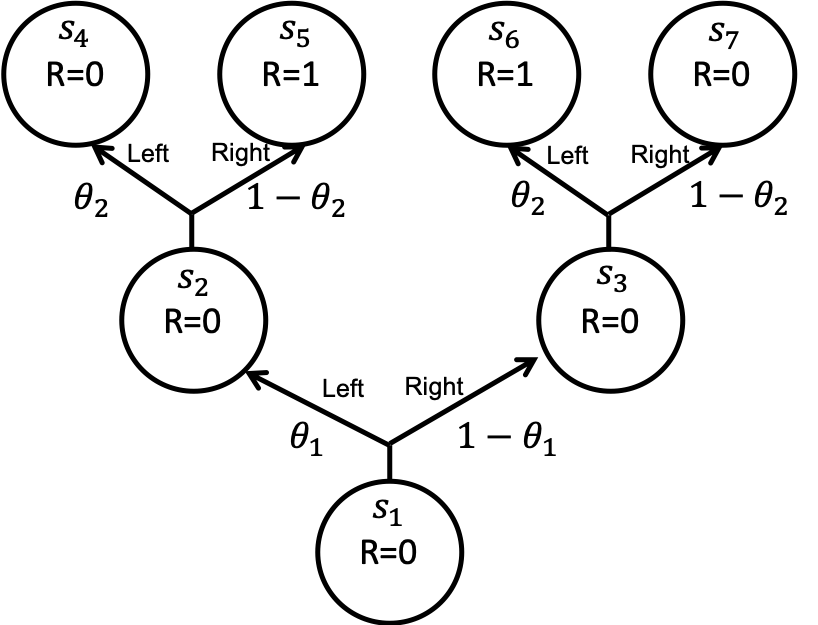
\includegraphics[width=0.5\textwidth]{figures/policy_diff.png}
    \caption{Example MDP}
    \label{fig:policy-diff-example}
\end{figure}

Intuitively, we expect that if the difference $\pi' - \pi$ is `small', then the difference in the state visitation frequencies $\discdist^{\policy'} - \discdist^{\policy}$ would also be `small', allowing us to safely replace $\discdist^{\policy'}$ in the right hand side of Eq.~\ref{eq:policy_perf_diff} with $\discdist^{\policy}$. This is the route taken by several algorithmic approaches, which differ in the way of defining a `small' policy perturbation. Of particular interest to us is the case of an infinitesimal perturbation, that is, the \textit{policy gradient} $\nabla_{\theta} J(\theta)$. In the following, we shall describe in detail several algorithms for estimating the policy gradient.

% \begin{theorem}\label{thm:policy_gradient_direct}
%     We have that
%     \begin{equation*}
%         \nabla J(\theta) = \sum_{\state} \discdist^{\policy}(\state) \sum_\action \nabla \policy(\action|\state)\QValue^{\policy}(\state,\action).
%     \end{equation*}
% \end{theorem}
% \begin{proof}
%     For simplicity we consider that $\theta$ is a scalar; the extension to the vector case is immediate.
%     By definition we have that
%     \begin{equation*}
%         \begin{split}
%             \frac{\partial J(\theta)}{\partial \theta} &= \lim_{\delta \theta \to 0} \frac{J(\theta+ \delta \theta) - J(\theta)}{\delta \theta} \\
%             &=\lim_{\delta \theta \to 0} \frac{\sum_{\state} \discdist^{\policy_{\theta+ \delta \theta}}(\state) \sum_\action \policy_{\theta+ \delta \theta}(\action|\state)\left( \QValue^{\policy_{\theta}}(\state,\action) - \Value^{\policy_{\theta}}(\state)\right)}{\delta \theta}\\
%             &= \lim_{\delta \theta \to 0} \frac{\sum_{\state} \discdist^{\policy_{\theta+ \delta \theta}}(\state) \sum_\action \left(\policy_{\theta+ \delta \theta}(\action|\state) - \policy_{\theta}(\action|\state)\right) \QValue^{\policy_{\theta}}(\state,\action)}{\delta \theta}\\
%             &= \sum_{\state} \discdist^{\policy}(\state) \sum_\action \frac{\partial \policy(\action|\state)}{\partial \theta} \QValue^{\policy}(\state,\action),
%         \end{split}
%     \end{equation*}
% where the second equality uses Lemma \ref{lemma:perf_diff} and the third equality is since $\Value^{\policy_{\theta}}(\state) = \sum_{\action} \policy_{\theta}(\action|\state) \QValue^{\policy_{\theta}}(\state,\action)$.
% \end{proof}


\section{Gradient-Based Policy Optimization}
We would like to use the policy gradient to optimize the expected
return  $J(\theta)$ of the policy $\policy(\cdot|\cdot,\theta)$. We
will compute the gradient of $J(\theta)$, i.e., $\nabla_\theta
J(\theta)$. The update of the policy parameter $\theta$ is by gradient ascent,
\[
\theta_{\ttime+1}=\theta_\ttime + \alpha \nabla_{\theta_\ttime}
J(\theta_\ttime),
\]
where $\alpha$ is a learning rate. For a small enough learning rate, each update is guaranteed to increase $J(\theta)$.

In the following, we shall explore several different approaches for calculating the gradient $\nabla_{\theta} J(\theta)$ using rollouts from the MDP.

% One challenge we will have to address is to relate the global gradient, $\nabla_\theta J(\theta)$, to the local gradients, $\nabla \policy(\action|\state,\theta)$.



\subsection{Finite Differences Methods}

These methods can be used even when we do not have a representation
of the gradient of the policy or even the policy itself. This may
arise many times when we have, for example, access to an
off-the-shelf robot for which the software is encoded already in the
robot. In such cases we can estimate the gradient by introducing
perturbations in the parameters.

The simplest case is component-wise gradient estimates, which is also named \emph{coordinate ascent} . Let $e_i$ be
a unit vector, i.e., has in the $i$-th entry a value $1$ and a value
$0$ in all the other entries. The perturbation that we will add is
$\delta e_i$ for some $\delta >0$. We will use the following
approximation:
\[
\frac{\partial}{\partial \theta_i}J(\theta)\approx
\frac{\hat{J}(\theta+\delta e_i)-\hat{J}(\theta)}{\delta}
\]
where $\hat{J}(\theta)$ is unbiased estimator of $J(\theta)$. A more
symmetric approximation is sometimes better,
\[
\frac{\partial}{\partial \theta_i}J(\theta)\approx
\frac{\hat{J}(\theta+\delta e_i)-\hat{J}(\theta-\delta e_i
)}{2\delta}
\]

The problem is that we need to average many samples of
$\hat{J}(\theta\pm\delta e_i)$ to overcome the noise. Another
weakness is that we need to do the computation per dimension. In
addition, the selection of $\delta$ is also critical. A small
$\delta$ might have a large noise rate that we need to overcome (by
using many samples). A large $\delta$ run the risk of facing the
non-linearity of $J$.

Rather then performing separately the computation and optimization per dimension, we can perform a more global approach and use a least squares estimation of the gradient.
Consider a random vector $u_i$, then we have
\[
J(\theta+\delta u_i)\approx J(\theta)+\delta u_i^\top \nabla
J(\theta) \;.
\]
We can define the following least square problem,
\[
G= \arg\min_x \sum_i (J(\theta+\delta u_i)- J(\theta)-\delta
u_i^\top x)^2,
\]
where $G$ is our estimate for $\nabla J(\theta)$.

We can reformulate the problem in matrix notation and define $\Delta
J^{(i)}=J(\theta+\delta u_i)- J(\theta)$ and $\Delta J= [\cdots ,
\Delta J^{(i)}, \cdots]^\top$. We define $\Delta \theta^{(i)}=\delta
u_i$, and the matrix $[\Delta\Theta]=[\cdots
\Delta\theta^{(i)},\cdots]^\top$, where the $i$-th row is
$\Delta\theta^{(i)}$.

We would like to solve for the gradient, i.e,
\[
\Delta J\approx [\Delta \Theta]x\;.
\]
This is a standard least square problem and the solution is
\[
G=([\Delta \Theta]^\top [\Delta \Theta])^{-1} [\Delta\Theta]^\top
\Delta J\;.
\]

One issue that we neglected is that we actually do not a have the
value of $J(\theta)$. The solution is to solve also for the value of
$J(\theta)$.
%
We can define a matrix $M=[1, [\Delta\Theta]]$, i.e., adding a column of ones, a vector of unknowns $x=[J(\theta), \nabla J(\theta)]$, and have the target be $z=[\cdots, J(\theta+\delta u_i),\cdots]$. We can now solve for $z\approx Mx$, and this will recover an estimate also for $J(\theta)$.


\section{Policy Gradient Theorem}

The policy gradient theorem will relate the gradient of the expected
return $\nabla J(\theta)$ and the gradients of the policy $\nabla
\policy(\action|\state,\theta)$. We make the following assumption.
\begin{assumption}\label{ass:differentiable_policy}
The gradient $\nabla
\policy(\action|\state,\theta)$ exists and is finite for every $\theta \in \mathbb{R}^d$, $\state \in \States$, and $\action \in \Actions$.
\end{assumption}

We will mainly try to make sure
that we are able to use it to get estimates, and the quantities
would be indeed observable by the learner.

\begin{theorem}\label{thm:policy_gradient_direct}
    Let Assumption \ref{ass:differentiable_policy} hold. We have that
    \begin{equation*}
        \nabla J(\theta) = \sum_{\state} \discdist^{\policy}(\state) \sum_\action \nabla \policy(\action|\state)\QValue^{\policy}(\state,\action).
    \end{equation*}
\end{theorem}
\begin{proof}
    For simplicity we consider that $\theta$ is a scalar; the extension to the vector case is immediate.
    By definition we have that
    \begin{equation*}
        \begin{split}
            \frac{\partial J(\theta)}{\partial \theta} &= \lim_{\delta \theta \to 0} \frac{J(\theta+ \delta \theta) - J(\theta)}{\delta \theta} \\
            &=\lim_{\delta \theta \to 0} \frac{\sum_{\state} \discdist^{\policy_{\theta+ \delta \theta}}(\state) \sum_\action \policy_{\theta+ \delta \theta}(\action|\state)\left( \QValue^{\policy_{\theta}}(\state,\action) - \Value^{\policy_{\theta}}(\state)\right)}{\delta \theta}\\
            &= \lim_{\delta \theta \to 0} \frac{\sum_{\state} \discdist^{\policy_{\theta+ \delta \theta}}(\state) \sum_\action \left(\policy_{\theta+ \delta \theta}(\action|\state) - \policy_{\theta}(\action|\state)\right) \QValue^{\policy_{\theta}}(\state,\action)}{\delta \theta}\\
            &= \sum_{\state} \discdist^{\policy}(\state) \sum_\action \frac{\partial \policy(\action|\state)}{\partial \theta} \QValue^{\policy}(\state,\action),
        \end{split}
    \end{equation*}
\sloppy where the second equality uses Lemma \ref{lemma:perf_diff} and the third equality is since $\sum_\action \policy_{\theta+ \delta \theta}(\action|\state)\Value^{\policy_{\theta}}(\state) = \Value^{\policy_{\theta}}(\state)$, and $\Value^{\policy_{\theta}}(\state) = \sum_{\action} \policy_{\theta}(\action|\state) \QValue^{\policy_{\theta}}(\state,\action)$. The fourth equality holds by definition of the derivative, and using Assumption \ref{ass:differentiable_policy}. Note that Assumption \ref{ass:differentiable_policy} guarantees that $\policy$ is continuous in $\theta$, and therefore $P^{\policy}$ is continuous in $\theta$, and by Proposition \ref{prop:visitation_freq} we must have $\lim_{\delta \theta \to 0} \discdist^{\policy_{\theta+ \delta \theta}}(\state) = \discdist^{\policy}(\state)$.
\end{proof}

The Policy Gradient Theorem gives us a way to compute the gradient.
We can sample states from the distribution $\discdist^{\policy}(\state)$ using the
policy $\policy$. We still need to resolve the sampling of the
action. We are going to observe the outcome of only one action in
state $\state$, and the theorem requires summing over all of them!
In the following we will slightly modify the theorem so that we will
be able to use only the action $\action$ selected by the policy
$\policy$, rather than summing over all actions.

Consider the following simple identity,
\[
\nabla f(x)=f(x)\frac{\nabla f(x)}{f(x)}=f(x)\nabla \log f(x)
\]
This implies that we can restate the Policy Gradient Theorem as the
following corollary,
\begin{corollary}[Policy Gradient Corollary] 
\label{thm:policy-gradient-corr} Consider a random rollout from the policy $\state_0,\action_0,\reward_0,\dots,\state_\termtime, \action_\termtime, \reward_\termtime$, where $\state_0 \sim \initdist$, $\action_\ttime\sim \policy(\cdot|\state_\ttime,\theta)$, $\state_{\ttime+1} \sim \transitionkernel (\cdot | \state_\ttime, \action_\ttime)$, and $\termtime$ is the termination time. We have
\begin{equation*}
\begin{split}
\nabla J(\theta) &= \sum_{\state \in \States} \discdist^{\policy}(\state) \sum_{\action\in
\Actions} \policy(\action|\state) \QValue^\policy
(\state,\action) \nabla \log \policy(\action|\state) \\
&=\mathbb{E}^\policy\left[\sum_{\ttime=0}^{\tau}\QValue^\policy (\state_\ttime,\action_\ttime)\nabla \log
\policy(\action_\ttime|\state_\ttime)\right].    
\end{split}
\end{equation*}
\end{corollary}
\begin{proof}
    The first equality is by the identity above, and the second is by definition of $\discdist^{\policy}(\state)$.
\end{proof}
Note that in the above corollary both the state $\state$ and action
$\action$ are sampled using the policy $\policy$. This avoids the need to sum over all actions, and leaves only the action selected by the policy.

We next provide some examples for the policy gradient theorem.

\begin{example}
Consider an MDP with a single state $\state$ (which is also called
Multi-Arm Bandit)
% , and is discussed in Chapter \ref{chapter:MAB}).
Assume we have only two actions, action $\action_1$ has expected
reward $\reward_1$ and action $\action_2$ has expected reward
$\reward_2$.

The policy $\policy$ is define with a parameter
$\theta=(\theta_1,\theta_2)$, where $\theta_i\in \reals$. Given
$\theta$ the probability of action $\action_i$ is
$p_i=e^{\theta_i}/(e^{\theta_1}+e^{\theta_2})$. We will also select
a horizon of length one, i..e, $\tHorizon=1$. This implies that
$\QValue^\policy(\state,\action_i)=\reward_i$.

In this simple case we can compute directly $J(\theta)$ and $\nabla
J(\theta)$. The expected return is simply,
\[
J(\theta)=p_1 \reward_1 + p_2 \reward_2 =
\frac{e^{\theta_1}}{e^{\theta_1}+e^{\theta_2}} \reward_1 +
\frac{e^{\theta_2}}{e^{\theta_1}+e^{\theta_2}} \reward_2
\]
Note that $\frac{\partial}{\partial \theta_1} p_1=
p_1-p_1^2=p_1(1-p_1) $ and $\frac{\partial }{\partial \theta_2} p_1=
- p_1 p_2= -p_1(1-p_1)$. The gradient is
\[
\nabla J(\theta)= \reward_1 \begin{pmatrix} p_1(1-p_1)\\
-p_1(1-p_1)\end{pmatrix} + \reward_2 \begin{pmatrix} -p_1(1-p_1)\\
p_1(1-p_1)\end{pmatrix} = (\reward_1-\reward_2) p_1(1-p_1) \begin{pmatrix}+1\\
-1\end{pmatrix}
\]
Updating in the direction of the gradient, in the case that
$\reward_1>\reward_2$, would increase $\theta_1$ and decrease
$\theta_2$, and eventually $p_1$ will converge to $1$.

To apply the Policy gradient theorem we need to compute the
gradient,
\[
\nabla_\theta \policy(\action_1|\state;\theta) = \nabla \begin{pmatrix} p_1\\
1-p_1\end{pmatrix}=  \begin{pmatrix} p_1(1-p_1)\\
-p_1(1-p_1)\end{pmatrix}
\]
and the policy gradient theorem gives us the same expression,
\[
\nabla J(\theta) = \reward_1 \nabla
\policy(\action_1;\theta)+\reward_2 \nabla
\policy(\action_2;\theta)=\reward_1 \begin{pmatrix} p_1(1-p_1)\\
-p_1(1-p_1)\end{pmatrix} + \reward_2 \begin{pmatrix} -p_1(1-p_1)\\
p_1(1-p_1)\end{pmatrix}
\]
where we used the fact that there is only a single state $\state$,
and that $\QValue^\policy(\state,\action_i)=\reward_i$.
\end{example}

\begin{example}
Consider the following deterministic MDP. We have states
$\States=\{\state_0,\state_1,\state_2,\state_3\}$ and actions
$\Actions=\{\action_0,\action_1\}$. We start at $\state_0$. Action
$\action_0$ from any state leads to $\state_3$. Action $\action_1$
moves from $\state_0$ to $\state_1$, from $\state_1$ to $\state_2$ and from $\state_2$ to $\state_3$. All the rewards are zero except the terminal reward at
$\state_2$ which is $1$. The horizon is $\tHorizon=2$. This implies
that the optimal policy performs in each state $\action_1$ and has a
return of $1$.

We have a log-linear policy parameterized by $\theta\in\reals^4$. In
state $\state_0$ it selects action $\action_1$ with probability
$p_1=e^{\theta_1}/(e^{\theta_1}+e^{\theta_2})$, and in state
$\state_1$ it selects action $\action_1$ with probability
$p_2=e^{\theta_3}/(e^{\theta_3}+e^{\theta_4})$.

For this simple MDP we can specify the expected return
$J(\theta)=p_1p_2$. We can also compute the gradient and have
\[
\nabla J(\theta)=\begin{pmatrix}p_1(1-p_1)p_2\\
-p_1(1-p_1)p_2 \\  p_1 p_2 (1-p_2) \\ -p_1 p_2 (1-p_2)\end{pmatrix}= p_1 p_2\begin{pmatrix}(1-p_1)\\
-(1-p_1) \\  (1-p_2) \\ - (1-p_2)\end{pmatrix}
\]

The policy gradient theorem will use the following ingredients. The
$\QValue^\policy$ is: $\QValue^\policy(\state_0,\action_1)=p_2$,
$\QValue^\policy(\state_1,\action_1)=1$ and all the other entries are
zero. The weights of the states are $\discdist^{\policy}(\state_0)=1$,
$\discdist^{\policy}(\state_1)=p_1$, $\discdist^{\policy}(\state_2)=p_1 p_2$ and
$\discdist^{\policy}(\state_3)=2-p_1-p_1 p_2$. The gradient of the action in each
state is:
\[
\nabla \policy(\action_1|\state_0;\theta)=
p_1\begin{pmatrix}1\\0\\0\\0\end{pmatrix} - p^2_1
\begin{pmatrix}1\\0\\0\\0\end{pmatrix} - p_1(1-p_1)
\begin{pmatrix}0\\1\\0\\0\end{pmatrix} = p_1(1-p_1)\begin{pmatrix}1\\-1\\0\\0\end{pmatrix}
\]
Similarly
\[
\nabla \policy(\action_1|\state_1;\theta)=
p_2\begin{pmatrix}0\\0\\1\\0\end{pmatrix} - p_2^2
\begin{pmatrix}0\\0\\1\\0\end{pmatrix} - p_2(1-p_2)
\begin{pmatrix}0\\0\\0\\1\end{pmatrix} = p_2(1-p_2)\begin{pmatrix}0\\0\\1\\-1\end{pmatrix}
\]
The policy gradient theorem states that the expected return gradient
is

\[
\discdist^{\policy}(\state_0)\QValue^\policy(\state_0,\action_1)\policy(\action_1|\state_0;\theta)
\nabla \log \policy(\action_1|\state_0;\theta) +
\discdist^{\policy}(\state_1)\QValue^\policy(\state_1,\action_1)\policy(\action_1|\state_1;\theta)
\nabla \log \policy(\action_1|\state_1;\theta)
\]

where we dropped all the terms that evaluate to zero. plugging in
our values we have
\[
p_2 p_1 (1-p_1)\begin{pmatrix}1\\-1\\0\\0\end{pmatrix} + p_1 p_2
(1-p_2)\begin{pmatrix}0\\0\\1\\-1\end{pmatrix} = p_1 p_2\begin{pmatrix}(1-p_1)\\
-(1-p_1) \\  (1-p_2) \\ - (1-p_2)\end{pmatrix}
\]
which is identical to $\nabla J(\theta)$.
\end{example}

\begin{example}
    Consider the bandit setting with continuous action, where the MDP has only a single state and the horizon is $T=1$. The policy and reward are given as follows:
\begin{equation*}
    \begin{split}
        r(u) &= u, \\
        \pi_\theta(u) &= \frac{1}{\sqrt{2 \pi \sigma^2}} \exp (- \frac{(u - \theta)^2}{2 \sigma^2}).
    \end{split}
\end{equation*}
We have that $J(\theta) = \mathbb{E}[u] = \theta$, and thus $\nabla_\theta J(\theta) = 1.$
Using the policy gradient formula, we calculate:
\begin{equation*}
    \begin{split}
        \nabla_\theta \log \pi_\theta(u) &= \frac{u - \theta}{\sigma^2}, \\
        \nabla_\theta J(\theta) &= \mathbb{E} \left[\frac{u(u - \theta)}{\sigma^2}\right] \\
        &= \frac{1}{\sigma^2} (\mathbb{E} [u^2] - (\mathbb{E} [u])^2) = 1.
    \end{split}
\end{equation*}
Note the intuitive interpretation of the policy gradient here: we average the change to the mean action $u-\theta$ and the reward it produces $r(u)=u$. In this case, actions above the mean lead to higher reward, thereby `pushing' the mean action $\theta$ to increase. 
\end{example}

\subsection{Alternative Proofs for the Policy Gradient Theorem}
In this section, for didactic purposes, we show two alternative proofs for the policy gradient theorem (Theorem \ref{thm:policy_gradient_direct}). The first proof is based on unrolling the Q value according to the Bellman equation.

\begin{proof}
For each state $\state$ we have
\begin{align*}
\nabla \Value^\policy(\state) =& \nabla \sum_\action \policy(\action|\state) \QValue^\policy(\state,\action)\\
=&\sum_\action  \QValue^\policy(\state,\action) \nabla \policy(\action|\state) + \policy(\action|\state) \nabla \QValue^\policy(\state,\action)\\
=&\sum_\action  \QValue^\policy(\state,\action) \nabla \policy(\action|\state) + \policy(\action|\state) \sum_{\state_1} \transitionkernel(\state_1|\state,\action) \nabla \Value^\policy(\state_1)\\
=& \sum_\action  \QValue^\policy(\state,\action) \nabla
\policy(\action|\state) + \sum_{\state_1} P^{\policy}(\state_1|\state)
\nabla \Value^\policy(\state_1)\\
=& \sum_\action  \QValue^\policy(\state,\action) \nabla
\policy(\action|\state) + \sum_{\state_1} P^{\policy}(\state_1|\state)
\sum_\action \QValue^\policy(\state_1,\action) \nabla
\policy(\action|\state_1) \\
& + \sum_{\state_1, \state_2}
P^{\policy}(\state_2|\state_1)P^{\policy}(\state_1|\state)
\nabla \Value^\policy(\state_2)\\
=& \sum_{\state\in
\States}\sum_{t=0}^\infty P(\state_t = \state | \state_0 = \state, \policy) \sum_\action
\QValue^\policy(\state,\action)\nabla\policy(\action|\state)
\end{align*}
where the first identity follows since by averaging $Q^\policy(\state,\action)$ over the actions $\action$, with the
probabilities induce by $\policy(\action|\state)$, we have both correct expectation of the immediate reward and the next state is distributed correctly. The second equality follows from the gradient of a multiplication, i.e., $\nabla AB=A\nabla B+B\nabla A$. The third follows since 
$\nabla \QValue^\policy(\state,\action)= \nabla
[\reward(\state,\action)+
\sum_{\state'}\transitionkernel(\state'|\state,\action)\Value^\policy(\state'|\state,\action)]$.
%
The next two identities role the policy one step in to the future.
%
The last identity follows from unrolling $\state_1$ to $\state_2$ etc., and then reorganizing the terms. The term that depends on $\nabla \Value^\policy(\state_2)$ for $t\to\infty$ because we assume that the termination time is bounded with probability 1.

Using this we have
\begin{align*}
\nabla J(\theta) &= \nabla \sum_{\state} \initdist(\state) \Value^\policy (\state)\\
&= \sum_\state \initdist(\state) \left(\sum_{t=0}^\infty P(\state_t = \state | \state_0 = \state, \policy) \right) \sum_\action \QValue^\policy (\state,\action) \nabla\policy(\action|\state) \\
&= \sum_\state \left(\sum_{t=0}^\infty P(\state_t = \state | \initdist, \policy) \right) \sum_\action \QValue^\policy (\state,\action) \nabla\policy(\action|\state) \\
&= \sum_\state \discdist^{\policy}(\state) \sum_\action \nabla\policy(\action|\state) \QValue^\policy (\state,\action) \\
\end{align*}
where the last equality is by definition of $\discdist^{\policy}$.
\end{proof}

The second 

\subsection{Policy Gradient Algorithms}




We can now apply the policy gradient to some simple policy
class. For the log-linear policy class we have $\log
\policy(\action|\state)\propto \phi(\state,\action)^\top \theta$,
and then
\[
\nabla \log \policy(\action|\state;\theta)= \phi(\state,\action) - \policy(\action|\state;\theta)\phi(\state,\action)\propto \phi(\state,\action)
%-\sum_b \policy(b|\state;\theta) \phi(\state,b)
\]
and the update is $\Delta\theta \propto \alpha U
\phi(\state,\action)$ where $E[U]=Q^\policy(\state,\action)$.
%and$v=\sum_b \policy(b|\state;\theta) \phi(\state,b)$.
%\footnote{We have $\log \policy(\action|\state;\theta) =  $}

For Gaussian policy class we have $\nabla \log
\policy(\action|\state;\theta)\propto
(\action-\mu(\state))\phi(\state)/\sigma^2$ and update is
$\Delta\theta \propto \alpha U
(\action-\mu(\state))\phi(\state)/\sigma^2$ where
$E[U]=Q^\policy(\state,\action)$.




The main benefit of the policy gradient theorem is that we do not
need to compute either $\mu(\state)$ or $Q^\policy$. We simply run
policy $\policy$ which visits each state $\state$ an expected
 $\mu(\state)$ times, and let $\policy$ select
actions. We substitute for $Q^\policy$ and unbiased random variable
with the same value. The only thing that we need to explicitly
compute is the gradient $\nabla \policy(\action|\state;\theta)$
which depends on our parametrization. In the next section we couple
the policy gradient theorem with Monte-Carlo updates to derive the
REINFORCE algorithm.


\section{REINFORCE: Monte-Carlo updates}

The REINFORCE algorithm uses Monte-Carlo updates in conjunction
with the policy gradient computation. Given an episode
$(\state_1,\action_1,\reward_1, \ldots ,
\state_T,\action_T,\reward_T)$ for each $\ttime\in [1,T]$ updates,

\[
\theta\leftarrow \theta+\alpha R_{\ttime:T} \nabla \log
\policy(\action_\ttime|\state_\ttime;\theta)
\]

where $R_{\ttime:T}=\sum_{i=\ttime}^T \reward_i$. (We are using here
every-visit updates, however, since we have a large state space, it
is likely that we never observe the same state twice.)


\subsection*{Baseline function}
We can extend the REINFORCE to add a baseline function.
The baseline function $b(\state)$ can depend in an arbitrary way on
the state, but does not depend on the action. The main observation
would be that we can add or subtract any such function from our
estimate $U$, and it will still be unbiased. This follows since
\[
\sum_\action b(\state) \nabla
\policy(\action|\state;\theta)=b(\state)\nabla \sum_\action
\policy(\action|\state;\theta)=b(\state)\nabla 1=0
\]
Given this, we can restate the Policy Gradient Theorem as,
\[
\nabla J(\theta)\propto \sum_{s\in S} \mu(\state) \sum_{\action\in
\Actions} (Q^\policy (\state,\action)-b(\state))\nabla_\theta
\policy(\action|\state;\theta)
\]
This gives us a degree of freedom to select $b(\state)$. Note that
by setting $b(\state)=0$ we get the original theorem. In many cases
it is reasonable to use for $b(\state)$ the value of the state,
i.e., $b(\state)=\Value^\policy(\state)$. The motivation for this is
to reduce the variance of the estimator. If we assume that the
magnitude of the gradients $\|\nabla
\policy(\action|\state;\theta)\|$ is similar for all actions
$\action\in \Actions$, we are left with $E^\policy
[(Q^\policy(\state,\action)-b(\state))^2]$ which is minimized by
$b(\state)=E^\policy[Q^\policy(\state,\action)]=\Value^\policy(\state)$.

We are left with the challenge of approximating
$\Value^\policy(\state)$. On the one hand this is part of the
learning. On the other hand we have developed tools to address this
in the previous chapter on value function approximation (Chapter~\ref{chapter:function-approximation}). We can use
$\Value^\policy(\state)\approx V(\state;\weight)=b(\state)$. The
good news is that any $b(\state)$ will keep the estimator unbiased,
so we do not depend on $V(\state;\weight)$ to be unbiased.

We can now describe the REINFORCE algorithm with baseline function.
We will use a Monte-Carlo sampling to estimate
$\Value^\policy(\state)$ and this will define our function
$b(\state)$. We will update using $U-b(\state)$ where
$E[U]=Q^\policy(\state,\action)$. More specifically, our algorithm
will have a class of value approximation function $V(\cdot;\weight)$
and a parameterized policy $\policy(\cdot|\cdot;\theta)$, and in
addition to step size parameters, $\alpha,\beta>0$. Given an episode
$(\state_1,\action_1,\reward_1,
\ldots,\state_\tHorizon,\action_\tHorizon,\reward_\tHorizon)$ for each $\ttime\in [1,\tHorizon]$ we
compute the $R_{\ttime:\tHorizon}$ during the times $[\ttime,\tHorizon]$, i.e.,
$R_{\ttime:\tHorizon}=\sum_{i=\ttime}^\tHorizon \reward_i$. The error in time $\ttime$ is
$\Gamma_\ttime=R_{\ttime:\tHorizon}-V(\state_\ttime;\weight)$. The updates
are
\[
\Delta w=\alpha \Gamma_\ttime \nabla V(\state_\ttime;\weight)
\]
and
\[
\Delta \theta=\beta\Gamma_\ttime \nabla \log
\policy(\action_\ttime|\state_\ttime;\theta)
\]

We can extend this to handle also TD updates. We will use an
actor-critic algorithm (see Chapter~\ref{section:actor-critic}). We will use a $Q$-value updates for this
(but can be done similarly with $V$-values).

The critic maintains an approximate $Q$ function $Q(\state,\action;\weight)$. For each time $\ttime$ it defines the TD error to be $\Gamma_\ttime = \reward_\ttime +Q(\state_{\ttime+1},\action_{\ttime+1};\weight)-Q(\state_\ttime,\action_\ttime;\weight)$. The update will be $\Delta w=\alpha\Gamma_\ttime \nabla Q(\state_\ttime,\action_\ttime;\weight)$. The critic send the actor the TD error $\Gamma_\ttime$.

The actor maintains a policy $\policy$ which is parameterized by $\theta$. Given a TD error $\Gamma_\ttime$ it updates $\Delta \theta= \beta \Gamma_\ttime \nabla \log \policy(\action_\ttime|\state_\ttime;\theta)$. Then it selects $\action_{\ttime+1}\sim \policy(\cdot|\state_{\ttime+1};\theta)$.

We need to be careful in the way we select the function
approximation $Q(\cdot;\weight)$ since it might introduce a bias.
The following theorem identifies a special case which guarantee
thats we will not have such a bias.

Let the expected square error of $\weight$ is
\[
SE(\weight)=\frac{1}{2}E^\policy[(Q^\policy(\state,\action)-Q(\state,\action;\weight))^2]
\]

A value function is {\em compatible} if,
\[
\nabla_\weight Q(\state,\action;\weight)= \nabla_\theta
\policy(\action|\state;\theta)
\]


\begin{theorem}
Assume that $Q$ is compatible and $\weight$ minimizes $SE(\weight)$,
then,
\[
\nabla_\theta J(\theta)\propto E^\policy[Q(\state,\action;\weight)
\nabla \log \policy(\action|\state;\theta)]
\]
\end{theorem}

\begin{proof}
Since $\weight$ minimizes $SE(\weight)$ we have
\begin{align*}
0 & = \nabla_\weight SE(\weight)\\
&= \nabla_\weight E^\policy[(Q^\policy(\state,\action)-Q(\state,\action;\weight))^2]\\
&=
E^\policy[(Q^\policy(\state,\action)-Q(\state,\action;\weight))\nabla_\weight
Q(\state,\action;\weight)]
\end{align*}
Since $Q$ is compatible, we have $\nabla_\weight
Q(\state,\action;\weight)= \nabla_\theta
\policy(\action|\state;\theta)$ which implies,
\begin{align*}
0&=
E^\policy[(Q^\policy(\state,\action)-Q(\state,\action;\weight))\nabla_\theta
\log \policy(\action|\state;\theta)]
\end{align*}
and have
\begin{align*}
 E^\policy[Q^\policy(\state,\action)\nabla_\theta \log \policy(\action|\state;\theta)] = E^\policy[Q(\state,\action;\weight)\nabla_\theta \log \policy(\action|\state;\theta)]
\end{align*}
This implies that by substituting $Q$ in the policy gradient theorem
we have
\[
\nabla_\theta J(\theta) \propto E^\policy[Q(\state,\action;\weight)
\nabla \log \policy(\action|\state;\theta)]
\]
\end{proof}

We can summarize the various updates for the policy gradient as
follows:
\begin{itemize}
\item REINFORCE (which is a Monte-Carlo estimate) uses
$E^\policy[R_\ttime \nabla\log\policy(\action|\state;\theta) ]$.
\item Q-function with actor-critic uses
$E^\policy[Q(\action_\ttime|\state_\ttime;\weight)
\nabla\log\policy(\action|\state;\theta) ]$.
\item A-function with actor-critic uses
$E^\policy[A(\action_\ttime|\state_\ttime;\weight)
\nabla\log\policy(\action|\state;\theta) ]$, where
$A(\action|\state;\weight)=Q(\state,\action;\weight)-V(\state;\weight)$. The A-function is also called the \emph{Advantage function}.
\item TD with actor-critic uses
$E^\policy[\Gamma\nabla\log\policy(\action|\state;\theta) ]$, where
$\Gamma$ is the TD error.
\end{itemize}


\section{Bibliography Remarks}

% Part of the outline borrows from David Silver class notes and the
% the book of Sutton and Barto \cite{SuttonB98}.

Our exposition of the Policy Gradient Theorem follows \cite{SuttonMSM99}. Alternative formulations of the theorem appears in \cite{MarbachT01,MarbachT03} and \cite{BaxterB01}.

The introduction of the REINFORCE algorithm is from \cite{Williams92}, which introduced also the baseline functions. Convergence properties of the reinforce algorithm were studies in \cite{PhansalkarT95}.

The Grid world example follows the example from David Silver class notes \cite{SilverClass}.

The training of Aibo for RoboSoccer is by \cite{KohlS04}.
The work on AlphaGo is by \cite{SilverHMGSDSAPL16}.



Recall that Reinforcement Learning is concerned with learning optimal control policies by interacting with the environment. So far, we have focused on learning methods that rely on learning the value function, from which the optimal policy can be inferred.
Policy gradient methods take a different approach. Here a set of \textbf{policies} is directly parameterized by a continuous set of parameters, which are then optimized online. The basic algorithms use online gradient descent, hence achieve only local optimality in the parameter space.
% To allow efficient learning, the parameter vector should be of a reasonably low dimension. 
This also means that the set of possible policies is restricted, and might require a fair amount of prior knowledge for its effective definition. On the other hand, the restriction to a given set of policies simplifies the treatment of various aspects of the RL problem such as large or continuous state and action spaces. For these reasons, policy gradient methods are finding many applications in the area of robot learning.
Policy Gradient algorithms belong to a larger class of Policy Search algorithms. An extensive survey can be found in:
\begin{itemize}
  \item M. Deisenroth, G. Neumann and J. Peters, "A Survey on Policy Search for Robotics," Foundations and Trends in Robotics, Vol. 2, 2011, pp. 1-142.
\end{itemize}
%
%Contents:
%13.1  Problem Description
%13.2  Finite Difference Methods
%13.3  Likelihood Ratio Methods

\section{Problem Description}

We consider the standard MDP model in discrete time, with states  ${x_t} \in X$, actions ${u_t} \in U$, transition kernel $\{ p(x'|x,u)\} $ , rewards  ${R_t} = {r_t}({x_t},{u_t})$, and policies $\pi  \in \Pi $.

For concreteness, we consider an episodic (finite horizon) problem with the total return criterion, which is to be maximized:
\[{J^\pi } = {\mathbb E^{\pi ,{x_0}}}\left(\sum\limits_{t = 0}^T {{R_t}} \right).\]
Here ${x_0}$ is a given initial state. We may allow the final time $T$ to depend on the state (as in the Stochastic Shortest Path problem), as long as it is bounded.

We next assume that we are given parameterized set of policies: $\{ {\pi _\theta },\,\theta  \in \Theta \} $, where $\theta $ is an $I$-dimensional parameter vector. We also refer to this set as a policy representation. The representation is often application-specific and should take into account prior knowledge on the problem.

We assume the following:
\begin{itemize}
  \item The actions set $U$ is continuous - typically a subset of $\mathbb R^l$.
If the original action set is finite, we extend it to a continuous set by considering  random (mixed) actions.
  \item The parameter set $\Theta $ is a continuous subset of $\mathbb R^I$.
  \item The policy set $\{ {\pi _\theta },\,\theta  \in \Theta \} $ is smooth in $\theta $. In particular, assuming each ${\pi _\theta }$ is a stationary policy,  ${\pi _\theta }(x)$ is a continuous function of $\theta $ for each state $x$.
\end{itemize}

\paragraph{Policy representation:} Some common generic representations include:
\begin{itemize}
  \item Linear policies:
                                      $$u = {\pi _\theta }(x) = {\theta ^T}\phi (x),$$
where $\phi (x)$ is a suitable set of basis functions (or  feature vectors).
  \item Radial Basis Function Networks:
             $${\pi _\theta }(x) = {w^T}\phi (x),  \textrm{ with }  {\phi _i}(x) = \exp ( - {\textstyle{1 \over 2}}{(x - {\mu _i})^T}{D_i}(x - {\mu _i})),$$
where ${D_i}$ is typically a diagonal matrix. The vector $\theta $ of tunable parameters includes $w$ (the linear parameters), and possibly $({\mu _i})$ and $({D_i})$ (nonlinear parameters).
  \item Neural Networks. For example, a Multi-Layer Perceptron (MLP):
  $$
    {\pi _\theta }(x) = \psi(b_2 + w_2^T \psi(b_1 + {w_1^T}\phi (x))),
  $$
  where $\psi$ is a non-linear activation function (e.g., $\tanh$ or sigmoid) and the vector $\theta$ includes the weight and the bias terms ($w_1,w_2,b_1,b_2$) of the neural network. This can be seen as a generalization of the linear policy to include non-linearities.
  \item Logistic (a.k.a. softmax) functions: For a discrete (finite) action space, one can use the Boltzman-like probabilities
                           $${\pi _\theta }(u|x) = \exp (w_u^T\phi (x))/\sum\nolimits_{u'} {\exp (w_{u'}^T\phi (x)} ),$$
where  $\theta  = {({w_u})_{u \in U}}$. It is convenient to designate one of the actions as 'anchor', with ${w_u} = 0$.
\item Stochastic policies: in certain cases a stochastic policy is required for sufficient exploration of the system. This is typically modelled by adding noise to a deterministic policy. For example, in a linear policy with Gaussian noise:
$$
P(u|x) = {\pi _\theta }(u|x) \sim \mathcal{N}\left( {w ^T}\phi (x), \sigma \right),
$$
where the parameter vector $\theta$ contains $w$ and the covariance matrix $\sigma$.
\end{itemize}

In robotics, a parameterized path is often described through a parameterized dynamical system, the output of which is used as a reference input to a feedback controller.

\paragraph{Gradient Updates:}  Plugging in the parameter-dependent policy ${\pi _\theta }$ in ${J^\pi }$,  we obtain the parameter-dependent return function:
\[J(\theta ) = {J^{{\pi _\theta }}}.\]

We wish to find a parameter $\theta $ that maximizes $J(\theta )$, at least locally. We discuss two high-level approaches for this task.

\section{Search in Parameter Space}
In this approach, the problem is viewed as a black-box optimization of the function $J(\theta )$.
Black-box optimization (a.k.a. derivative free optimization) refers to optimization of an objective function through a black-box interface: the algorithm may only query the function $J(\theta )$ for a point $\theta$; gradient information or the explicit form of $J(\theta)$ are not known. 

In our setting, for each given value of the parameter vector $\theta $, we can simulate or operate the system with control policy ${\pi _\theta }$ and measure the return  $\hat J(\theta ) = \sum\nolimits_{t = 0}^T {{R_t}} $, which gives an estimate of the expected return $J(\theta )$. We note that for stochastic systems or policies, this estimate will be noisy.

Note: The search in parameter space approach ignores the structure of our problem, namely, that trajectories are the result of rolling out a policy in an MDP. Only the mapping between $\theta$ and the resulting cumulative reward is considered.

Many black-box optimization algorithms have been proposed in the literature. We describe several that have been popular in RL literature.

\subsection{Gradient Approximation}

These methods use function evaluations of $J(\theta )$ to approximate the gradient ${\nabla _\theta }J(\theta )$.
Given the gradient, we may consider a gradient ascent scheme, of the form
\begin{equation}\label{eq:grad_ascent_scheme}
{\theta _{k + 1}} = {\theta _k} + {\alpha _k}\,{\nabla _\theta }J({\theta _k}).
\end{equation}
Here  $({\alpha _k})$ is the gain (or learning rate) sequence, and
\[{\nabla _\theta }J(\theta ) = \frac{{\partial J(\theta )}}{{\partial \theta }}\]
is the gradient of the return function with respect to $\theta $.

It remains of course to determine how to compute the required gradient. We next outline two options.

Note: Whenever required, we assume without further mention that $J(\theta )$ is continuously differentiable, and that the expectation and derivative in its definition can be interchanged.

\subsubsection*{Finite Difference Methods}
Finite difference methods are among the most common and straightforward methods for estimating the gradient in a variety of applications.

Suppose that, for each given value of the parameter vector $\theta $, we can simulate or operate the system with control policy ${\pi _\theta }$ and measure the return  $\hat J(\theta ) = \sum\nolimits_{t = 0}^T {{R_t}} $, which gives an estimate of the expected return $J(\theta )$. We note that this estimate will be noisy when either the policy or the system contain random moves.

\paragraph{Component-wise gradient estimates:} We can now obtain a noisy estimate of each component of the gradient vector using a finite difference of the form:
\[\frac{{\partial J(\theta )}}{{\partial {\theta _i}}} \approx \frac{{\hat J(\theta  + \delta {e_i}) - \hat J(\theta )}}{\delta },\]
or, preferably, the symmetric difference
  \[\frac{{\partial J(\theta )}}{{\partial {\theta _i}}} \approx \frac{{\hat J(\theta  + \delta {e_i}) - \hat J(\theta  - \delta {e_i})}}{{2\delta }}.\]
\paragraph{Note:}
\begin{itemize}
  \item Since the estimates $\hat J$ are typically noisy, repeated trials and averaging of several such differences are needed to reduce the estimation error. However, one can also use the noisy estimates with a low gain in the gradient ascent scheme, which has a similar averaging effect.
  \item The choice of the step size $\delta $ is crucial, as it controls the tradeoff between the relative noise level and the non-linearity of $J(\theta )$. We will not get into this issue here.
  \item A useful method to reduce the variance of the above difference is to use coupled random simulation, meaning that the random variables that govern the random choices in the simulation (or action choices) are drawn only once, and used for both estimates $\hat J(\theta  + \delta {e_i})$ and $\hat J(\theta  - \delta {e_i})$. These and other variance reduction methods are standard tools in the area of Monte-Carlo simulation.
\end{itemize}

\paragraph{Least-squared gradient estimates:}  Suppose we simulates/operate the system with a set of parameters ${\theta ^{[k]}} = \theta  + \Delta {\theta ^{[k]}}$, $1 \le k \le K$, to obtain a corresponding set of reward estimates ${\hat J^{[k]}} = \hat J(\theta  + \Delta {\theta ^{[k]}})$.

We can now use the linear relations
\begin{equation}\label{eq:LS_grad}
    \hat J(\theta  + \Delta {\theta ^{[k]}}) \approx J(\theta ) + \Delta {\theta ^{[k]}} \cdot \nabla J(\theta )
\end{equation}
to obtain a least-squares estimate of $\nabla J(\theta )$. For example, if an estimate $\hat J(\theta )$ is pre-computed, the relation
\[\Delta {J^{[k]}} \buildrel \Delta \over = \hat J(\theta  + \Delta {\theta ^{[k]}}) - \hat J(\theta ) \approx \Delta {\theta ^{[k]}} \cdot \nabla J(\theta )\]
leads to the LS estimate
\[\hat \nabla J(\theta ) = {({\bf{\Delta }}{{\bf{\Theta }}^T}{\bf{\Delta \Theta }})^{ - 1}}{\bf{\Delta }}{{\bf{\Theta }}^T}{\bf{\Delta J}},\]
where ${\bf{\Delta \Theta }} = {[\Delta {\theta ^{[1]}}, \ldots ,\Delta {\theta ^{[K]}}]^T}$, and ${\bf{\Delta J}} = {[\Delta {J^{[1]}}, \ldots ,\Delta {J^{[K]}}]^T}$.  (Note that we consider here $\Delta {\theta ^{[k]}}$ as a column vector, so that ${\bf{\Delta \Theta }}$ is a $K \times I$ matrix).

If $\hat J(\theta )$ is not given in advance, we can use directly the relations from \eqref{eq:LS_grad} in matrix form,
\[{\bf{\hat J}} \buildrel \Delta \over = \left[ {\begin{array}{*{20}{c}}
{{{\hat J}^{[1]}}}\\
 \vdots \\
{{{\hat J}^{[K]}}}
\end{array}} \right] \approx M\left[ {\begin{array}{*{20}{c}}
{J(\theta )}\\
{\nabla J(\theta )}
\end{array}} \right],\quad \quad M = [{\bf{1}},{\bf{\Delta \Theta }}]\]
to obtain the joint estimate ${({M^T}M)^{ - 1}}M\,{\bf{\hat J}}$ for $J(\theta )$ and $\nabla J(\theta )$.

\section{Population Based Methods}

This family of methods maintain a distribution over the parameter vector $\theta$, and use function evaluations to `narrow in' the distribution on an optimal choice. Assume that we have a parametrized distribution over the policy parameters $P_\phi(\theta)$. Note the distinction between the policy parameters $\theta$ and the parameters $\phi$ for the distribution of $\theta$ values.

For example, $P_\phi(\theta)$ can be a multivariate Gaussian, where $\phi$ encodes the mean and covariance of the Gaussian. 

\paragraph{Cross Entropy Method (CEM)}
This method updates $\phi$ iteratively according to the following scheme:
\begin{enumerate}
    \item Given current parameter $\phi_i$, sample $N$ population members
    $$
    \theta_k \sim P_{\phi_i}(\theta), \quad k=1,\dots,N.
    $$
    \item For each $k$, simulate the system with ${\pi_{\theta_k} }$ and measure the return $J(\theta_k)$.
    \item Let $K^*$ denote a set of the $p$\% top performing parameters
    \item Improve the parameter: 
    \begin{equation*}
    \phi_{i+1} = \argmax_\phi \sum_{k \in K^*} \log P_{\phi}(\theta_k). 
    \tag{$\star$}
    \end{equation*}
\end{enumerate}
The intuition here is that by refitting the distribution $P_\phi$ to the top performing parameters in the population, we are iteratively improving the distribution.

Note that other forms of the improvement step ($\star$) have been proposed in the literature. For example, in Reward Weighted Regression (RWR) the parameters are updated according to $$\phi_{i+1} = \argmax_\phi \sum_{k \in 1,\dots,N} J(\theta_k)\log P_{\phi}(\theta_k).$$

\section{Likelihood Ratio Methods}
Likelihood ratio-based methods allow to obtain a (noisy) estimate of the reward gradient from a \textbf{single} trial. The approach is again standard in the Monte-Carlo simulation area, where it is also known as the Score Function methods. Its first use in the controlled process (or RL) context is known as the REINFORCE algorithm. Interestingly, the RL formulation of this method can exploit the MDP structure of the problem, by using dynamic programming ideas to reduce variance in the estimation. 

Let ${\bf{\tau }} = ({x_0},{u_0}, \ldots ,{x_T})$ denote the process history, or sample path, of a single run of our episodic problem.  For simplicity we consider here a discrete model (finite state and action sets). Let ${p_\theta }({\bf{\tau }})$ denote the probability mass function induced on the process by the policy ${\pi _\theta }$. That is, assuming ${\pi _\theta }$ is a Markov policy,
\[{p_\theta }({\bf{\tau }}) = p({x_0})\prod\limits_{t = 0}^{T - 1} {{\pi _\theta }({u_t}|{x_t})p({x_{t + 1}}|{x_t},{u_t})}. \]
Denote $R({\bf{\tau }}) = \sum\nolimits_{t = 0}^{T - 1} {r({x_t},{u_t}) + {r_T}({x_T})} $, so that
\[J(\theta ) = {\mathbb E^\theta }(R({\bf{\tau }})) = \sum\nolimits_{\bf{\tau }} {R({\bf{\tau }}){p_\theta }({\bf{\tau }})\,} .\]
Observe now that${\nabla _\theta }{p_\theta }({\bf{\tau }}) = {p_\theta }({\bf{\tau }})\,{\nabla _\theta }\log {p_\theta }({\bf{\tau }})$. Therefore, assuming that the expectation and derivative can be interchanged,
\begin{align*}
\nabla J(\theta ) &= \sum\nolimits_{\bf{\tau }} {R({\bf{\tau }}){\nabla _\theta }{p_\theta }({\bf{\tau }})} \\
 &= \sum\nolimits_{\bf{\tau }} {[R({\bf{\tau }}){\nabla _\theta }\log {p_\theta }({\bf{\tau }})]\,{p_\theta }({\bf{\tau }})} \\
 &= {\mathbb E^\theta }\left( {R({\bf{\tau }}){\nabla _\theta }\log {p_\theta }({\bf{\tau }})} \right).
\end{align*}
Furthermore, observing the above expression for ${p_\theta }({\bf{\tau }})$,
\[{\nabla _\theta }\log {p_\theta }({\bf{\tau }}) = \sum\limits_{t = 0}^{T - 1} {{\nabla _\theta }\log {\pi _\theta }({u_t}|{x_t})} .\]
Importantly, the latter expression depends only on the derivative of the control policy, which is known to us, and not on the (unknown) process dynamics and reward function.

We can now obtain an unbiased estimate of $\nabla J(\theta )$ as follows:
\begin{itemize}
  \item Simulate/implement a single episode ("rollout") of the controlled system with policy ${\pi _\theta }$.
  \item Compute $R({\bf{\tau }})$ as $R({\bf{\tau }}) = \sum\nolimits_{t = 0}^{T - 1} {r({x_t},{u_t}) + {r_T}({x_T})} $, or directly using the observed rewards $R({\bf{\tau }}) \buildrel \Delta \over = \sum\nolimits_{t = 0}^T {{R_t}} $.
  \item Compute   $\hat \nabla J(\theta ) = R({\bf{\tau }})\sum\limits_{t = 0}^{T - 1} {{\nabla _\theta }\log {\pi _\theta }({u_t}|{x_t})} $
This is typically a noisy estimate, which can of course be improved by averaging over repeated trials.
\end{itemize}

\subsubsection{Illustrative Example}



\subsection{Variance Reduction}
We now provide a generalization of the policy gradient. We will consider an episodic MDP setting, and assume that for every policy parameter $\theta$, an absorbing state is reached w.p.~1. We can therefore replace the finite horizon return with an infinite sum ${J^\pi } = {\mathbb E^{\pi ,{x_0}}} \left(\sum\limits_{t = 0}^\infty {{R_t}} \right)$. We also recall the value and action value functions $V^\pi(x)$ and $Q^\pi(x,u)$. 
\begin{proposition}\label{prop:pg_control_variates}
The policy gradient can be written as:
\begin{equation*}
    \nabla_\theta J(\theta) = {\mathbb E^\theta }\left( \sum_{t=0}^\infty \Psi_t {{\nabla _\theta }\log {\pi _\theta }({u_t}|{x_t})} \right),
\end{equation*}
where $\Psi_t$ can be either one of the following terms:
\begin{enumerate}
    \item Total reward, $\sum_{t=0}^\infty r(x_t,u_t) - b(x_t)$, where $b$ is a state-dependent baseline
    \item Future reward following action $u_{t}$, $\sum_{t'=t}^\infty r(x_{t'},u_{t'}) - b(x_{t'})$
    \item State-action value function, $Q^\pi(x_t,u_t)$
    \item Advantage function, $Q^\pi(x_t,u_t) - V^\pi(x_t)$
    \item Temporal difference, $r(x_t,u_t) + V^\pi(x_{t+1})- V^\pi(x_t)$
\end{enumerate}
\end{proposition}

All the above formulations are unbiased estimates of the policy gradient. However, they differ in their variance, and variance reduction plays an important role in practical applications\footnote{In the simulation literature, the technique of changing the variance of the estimate by adding terms that do not change its bias is known as \textit{control variates}.}. Let's illustrate this in the previous bandit example.

\subsubsection{Illustrative Example (cont'd)}
Consider the previous bandit setting, where we recall that
$        r(u) = u, \quad
        \pi_\theta(u) = \frac{1}{\sqrt{2 \pi \sigma^2}} \exp (- \frac{(u - \theta)^2}{2 \sigma^2}).$
Find a fixed baseline $b$ that minimizes the variance of the policy gradient estimate.

The policy gradient formula in this case is:
\begin{equation*}
        \nabla_\theta J(\theta) = \mathbb{E} \left[\frac{(u-b)(u - \theta)}{\sigma^2}\right] = 1, 
\end{equation*}
and we can calculate the variance
\begin{equation*}
\begin{split}
        \frac{1}{\sigma^4}\textrm{Var}\left[(u-b)(u - \theta)\right]  
        &=\frac{1}{\sigma^4}\mathbb{E}\left[\left((u-b)(u - \theta)\right)^2 - 1\right] \\
        &=\frac{1}{\sigma^4}\mathbb{E}\left[\left((u-\theta)(u - \theta) + (\theta-b)(u - \theta)\right)^2 - 1\right] \\
        &=\frac{1}{\sigma^4}\mathbb{E}\left[(u-\theta)^4 + 2(\theta-b)(u - \theta)^3 + (\theta-b)^2(u - \theta)^2 - 1\right] \\
        &=\frac{1}{\sigma^4}\mathbb{E}\left[(u-\theta)^4 + (\theta-b)^2(u - \theta)^2 - 1\right],
\end{split}
\end{equation*}
which is minimized for $b=\theta$.

\textbf{Note 1}: The average reward, state-action value function, and advantage function baselines are commonly used in practice. While in our illustrative example the average reward was optimal, in general it is not necessarily so. An in-depth discussion of this topic can be found in:  
\begin{itemize}
  \item Greensmith, E., Bartlett, P.L. and Baxter, J., 2004. Variance reduction techniques for gradient estimates in reinforcement learning. Journal of Machine Learning Research, 5(Nov), pp.1471-1530.
\end{itemize}
Nevertheless, these baselines often lead to significant performance gains in practice.

\textbf{Note 2}: Typically, the value functions $V^\pi$ and $Q^\pi$ will not be known, and will have to be estimated along with the policy gradient using TD methods or regression. An important question here is how the error in value function estimation affects the policy gradient bias. There exist special policy classes and function approximators that are said to be \textit{compatible}, where the value estimation error is orthogonal to the policy gradient bias. In general, however, this is not the case. 


\subsubsection{Proof of Proposition \ref{prop:pg_control_variates}}
\begin{proof}
We will start by establishing a useful property. 
Let $p_\theta(z)$ be some parametrized distribution. Differentiating $\sum\nolimits_{z } {{p_\theta }(z)}  = 1$  yields
\begin{equation}\label{eq:helper}
\sum\nolimits_{z} {(\nabla_\theta \log {p_\theta }({z})} ){p_\theta }({z}) = {\mathbb E^\theta }(\nabla_\theta  \log {p_\theta }({z})) = 0.
\end{equation}

We can now observe that adding a state-dependent baseline to the policy gradient does not add bias:
\begin{equation*}
\begin{split}
{\mathbb E^\theta }\left( \sum_{t=0}^\infty b(x_t) {{\nabla _\theta }\log {\pi _\theta }({u_t}|{x_t})} \right) &= \sum_{t=0}^\infty {\mathbb E^\theta }\left[ b(x_t) {{\nabla _\theta }\log {\pi _\theta }({u_t}|{x_t})} \right] \\ 
&= \sum_{t=0}^\infty {\mathbb E^\theta }\left[ {\mathbb E^\theta }\left[ \left. b(x_t) {{\nabla _\theta }\log {\pi _\theta }({u_t}|{x_t})} \right| x_t \right]\right] \\ 
&= \sum_{t=0}^\infty {\mathbb E^\theta }\left[ b(x_t) {\mathbb E^\theta }\left[ \left. {{\nabla _\theta }\log {\pi _\theta }({u_t}|{x_t})} \right| x_t \right]\right] \\ 
&= 0,
\end{split}
\end{equation*}
where the last equation follows from applying \eqref{eq:helper} to the inner expectation. Note that the justification for exchanging the expectation and infinite sum in the first equality is not straightforward. In this case it can be shown to hold by the Fubini theorem, using the assumption that every trajectory reaches a terminal state in a bounded time w.p.~1.

We continue to show the independence on past rewards. We have that
\begin{equation*}
\begin{split}
& {\mathbb E^\theta }\left[ \sum_{t=0}^\infty \sum_{t'=0}^{t-1} r(x_{t'},u_{t'}) {{\nabla _\theta }\log {\pi _\theta }({u_t}|{x_t})} \right] \\
&= \sum_{t=0}^\infty {\mathbb E^\theta }\left[ \sum_{t'=0}^{t-1} r(x_{t'},u_{t'}) {{\nabla _\theta }\log {\pi _\theta }({u_t}|{x_t})} \right] \\
&= \sum_{t=0}^\infty {\mathbb E^\theta }\left[ {\mathbb E^\theta }\left[ \left. \sum_{t'=0}^{t-1} r(x_{t'},u_{t'}) {{\nabla _\theta }\log {\pi _\theta }({u_t}|{x_t})} \right| x_0,u_0,\dots,x_t \right]\right] \\
&= \sum_{t=0}^\infty {\mathbb E^\theta }\left[ \sum_{t'=0}^{t-1} r(x_{t'},u_{t'}) {\mathbb E^\theta }\left[ \left. {{\nabla _\theta }\log {\pi _\theta }({u_t}|{x_t})} \right| x_0,u_0,\dots,x_t \right]\right] \\
&= \sum_{t=0}^\infty {\mathbb E^\theta }\left[ \sum_{t'=0}^{t-1} r(x_{t'},u_{t'}) {\mathbb E^\theta }\left[ \left. {{\nabla _\theta }\log {\pi _\theta }({u_t}|{x_t})} \right| x_t \right]\right] \\
&=0, 
\end{split}    
\end{equation*}
where in the second to last equality we used the Markov property, and in the last equality we again applied \eqref{eq:helper}. We have thus proved (1) and (2).

\textbf{Exercise 1:} where would this derivation fail for future rewards?
% Solution: the Markov property is required to obtain an expectation on P(u|x) which is the distribution of the policy, as required by \eqref{eq:helper}.

We continue to prove (3).
\begin{equation*}
\begin{split}
& {\mathbb E^\theta }\left[ \sum_{t=0}^\infty \sum_{t'=t}^{\infty} r(x_{t'},u_{t'}) {{\nabla _\theta }\log {\pi _\theta }({u_t}|{x_t})} \right] \\
& \sum_{t=0}^\infty {\mathbb E^\theta }\left[ \sum_{t'=t}^{\infty} r(x_{t'},u_{t'}) {{\nabla _\theta }\log {\pi _\theta }({u_t}|{x_t})} \right] \\
& \sum_{t=0}^\infty {\mathbb E^\theta }\left[ {\mathbb E^\theta }\left[ \left. \sum_{t'=t}^{\infty} r(x_{t'},u_{t'}) {{\nabla _\theta }\log {\pi _\theta }({u_t}|{x_t})}\right| x_t, u_t\right] \right] \\
& \sum_{t=0}^\infty {\mathbb E^\theta }\left[ {{\nabla _\theta }\log {\pi _\theta }({u_t}|{x_t})} {\mathbb E^\theta }\left[ \left. \sum_{t'=t}^{\infty} r(x_{t'},u_{t'}) \right| x_t, u_t\right] \right] \\
& \sum_{t=0}^\infty {\mathbb E^\theta }\left[ {{\nabla _\theta }\log {\pi _\theta }({u_t}|{x_t})} Q^\pi(x_t,u_t) \right]. \\
\end{split}    
\end{equation*}

\textbf{Exercise 2:} Prove (4) and (5).

\end{proof}

\subsection{Natural Policy Gradient}
In the gradient ascent scheme \eqref{eq:grad_ascent_scheme}, the idea is to take small steps that iteratively improve the policy. The question is, what is the best metric to define `small steps' in?
Taking a step $\eta$ in the gradient direction is equivalent to solving the following optimization problem:
\begin{equation}\label{eq:grad_descent_opt}
    \begin{split}
        \argmax_{\Delta \theta}&\quad \Delta \theta^\top \nabla J(\theta), \\
        s.t. &\quad \Delta \theta^\top \Delta \theta \leq \eta.
    \end{split}
\end{equation}
Thus, standard gradient ascent takes a small improvement step w.r.t.~a Euclidean distance in the parameter space. However, this scheme can be highly sensitive to the specific parametrization employed - it might be that a small change in parameters causes a very drastic change to the behavior of the policy. The natural gradient attempts to rectify this situation by replacing the Euclidean distance between two parameters $\theta $  and $\theta+\Delta\theta$ by the Kullback-Leibler distance\footnote{The Kullback–Leibler (KL) distance between two distributions $P,Q$ is defined as $D_{KL}(P||Q) = \sum_{x}P(x)\log \frac{P(x)}{Q(x)}$. It is a standard tool in information theory.} between the probability distributions ${p_\theta }({\bf{\tau }})$ and ${p_{\theta+\Delta\theta}}({\bf{\tau }})$ induced by these parameters. Using a Taylor expansion, the KL distance can be approximated as 
\begin{equation*}
    D_{KL}({p_\theta }({\bf{\tau }})||{p_{\theta+\Delta\theta}}({\bf{\tau }})) \approx \Delta \theta^\top F_\theta \Delta \theta,
\end{equation*}
where $F_\theta$ is the Fisher Information Matrix, $F_\theta = \sum_\tau p_\theta(\tau) \nabla \log p_\theta(\tau) \nabla \log p_\theta(\tau)^\top.$

Replacing the constraint in \eqref{eq:grad_descent_opt} with $\Delta \theta^\top F_\theta \Delta \theta \leq \eta$ leads to a modified gradient definition known as the Natural Gradient: :
\[{\nabla ^N}J(\theta ) = F_{\theta}^{ - 1}\nabla J(\theta ).\]
% where $\nabla J$ is the standard gradient, and $F(\theta )$ is the Fisher Information Matrix:
% \begin{align*}
% F(\theta ) &= \sum\nolimits_{\bf{\tau }} {{p_\theta }({\bf{\tau }})} (\nabla \log {p_\theta }({\bf{\tau }})){(\nabla \log {p_\theta }({\bf{\tau }}))^T}\\
%  &= {\mathbb E_{{\bf{\tau }} \sim {p_\theta }}}\left( {(\nabla \log {p_\theta }({\bf{\tau }})){{(\nabla \log {p_\theta }({\bf{\tau }}))}^T}} \right).
% \end{align*}
Note that the Fisher Information Matrix can be calculated by sampling, since $\log p_\theta(\tau)$ only requires knowing the policy (as in the policy gradient derivation above). 
Natural policy gradient schemes lead in general to faster and more robust convergence to the optimal policy.

% \paragraph{Variations and improvements:}
% \begin{enumerate}
%   \item Baseline variance reduction:  A somewhat more general estimate for $\nabla J(\theta )$ can be obtained by subtracting a constant from$R({\bf{\tau }})$, namely
%                                       \[\hat \nabla J(\theta ) = (R({\bf{\tau }}) - b)\sum\limits_{t = 0}^{T - 1} {{\nabla _\theta }\log {\pi _\theta }({u_t}|{x_t})} .\]
% This estimate remains unbiased, as differentiating $\sum\nolimits_{\bf{\tau }} {{p_\theta }({\bf{\tau }})}  = 1$  yields
%                               \[\sum\nolimits_{\bf{\tau }} {(\nabla \log {p_\theta }({\bf{\tau }})} ){p_\theta }({\bf{\tau }}) = {\mathbb E^\theta }(\nabla \log {p_\theta }({\bf{\tau }})) = 0.\]
% A proper choice of the constant $b$ can however significantly reduce the variance.  The optimal value of  $b$ can itself be estimated from the data.
%   \item Natural Gradients:  The gradient $\nabla J(\theta )$ is highly sensitive to the specific parametrization employed, even if the set of policies ${\{ {\pi _\theta }\} _{\theta  \in \Theta }}$ is the same.
% For example, replacing the component ${\theta_1}$ of the parameter vector by $\theta_1' = 10\,\theta_1$ changes the gradient direction.
% The natural gradient attempts to rectify this situation by replacing the Euclidean distance between two parameters $\theta $  and $\theta '$ by an appropriate distances between the probability distributions ${p_\theta }({\bf{\tau }})$ and ${p_{\theta '}}({\bf{\tau }})$ induced by these parameters. This leads a modified gradient definition known as the Natural Gradient: :
% \[{\nabla ^N}J(\theta ) = F{(\theta )^{ - 1}}\nabla J(\theta ),\]
% where $\nabla J$ is the standard gradient, and $F(\theta )$ is the Fisher Information Matrix:
% \begin{align*}
% F(\theta ) &= \sum\nolimits_{\bf{\tau }} {{p_\theta }({\bf{\tau }})} (\nabla \log {p_\theta }({\bf{\tau }})){(\nabla \log {p_\theta }({\bf{\tau }}))^T}\\
%  &= {\mathbb E_{{\bf{\tau }} \sim {p_\theta }}}\left( {(\nabla \log {p_\theta }({\bf{\tau }})){{(\nabla \log {p_\theta }({\bf{\tau }}))}^T}} \right).
% \end{align*}
% Natural policy gradient schemes have been developed which estimate the natural gradient by observing the system. These algorithms lead in general to faster and more robust convergence to the optimal policy.
%   \item Q-Function based gradient estimates:   In stationary problems (infinite horizon or SSP), the variance of the gradient estimates can be improved significantly by using a modified expression which involves the Q-function. This formulation is therefore the most commonly used.
% Consider an SSP problem, where T is the arrival time to some set of states. Let ${Q^{{\pi _\theta }}}(x,u)$ denote the Q-function under the stationary policy ${\pi _\theta }$.  Then the following holds (the proof will be discussed in the Tirgul):
% \[{\nabla _\theta }J(\theta ) = {\mathbb E^\theta }\sum\limits_{t = 0}^{T - 1} {({\nabla _\theta }\log {\pi _\theta }({u_t}|{x_t})){Q^{{\pi _\theta }}}({x_t},{u_t})} .\]
% This expression is known as the \emph{policy gradient theorem}. It can be used to estimate the gradient, by running in parallel an (independent) algorithm for estimating Q.
% \end{enumerate}
